\section{Web Interface}
Das Web-Interface ist nicht essenziell für das gelingen der Arbeit. Die Funktion des Web-Interface ist lediglich die Demonstration des Produkts. Durch das Web-Interface wird die Software wortwörtlich praktisch und das Prinzip verständlich. Der Nutzer nimmt direkt im Browser eine kurze Audioaufnahme auf, lädt diese hoch zum Server, und dieser antwortet mit der geschätzten Sprache. Bevor man die Aufnahme hochlädt kann man sie optional selbst abspielen.
\\
Die meisten modernen Geräte werden unterstützt. Theoretisch bedarf es dafür nur einen Internetanschluss und einem Mikrofon. 


\subsection{Frontend}
\begin{figure}[hbt]
	\centering
		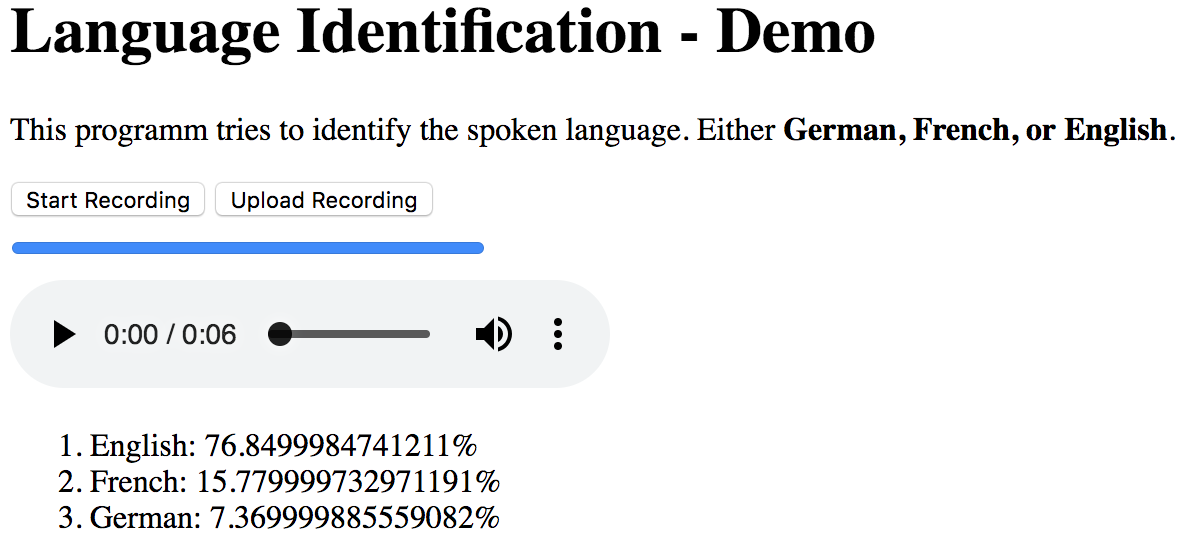
\includegraphics[width=0.6\textwidth]{assets/interface.png}
	\caption{Web-Interface Screenshot}
	\label{img:interface}
\end{figure}
Das Design ist in einfachem \textit{HTML} und \textit{CSS} geschrieben, die Logik mit \textit{Javascript}. Um im Browser Audioaufnahmen nehmen zu können, wird \textit{RecordRTC}\cite{recordrtc} verwendet. \textit{RecordRTC} ist eine unter der \textit{MIT} Lizenz veröffentlichte \textit{Javascript} Bibliothek für Medienaufnahmen. Sie ist kompatibel mit vielen modernen Browsern und Geräten.

Nach der Aufnahme wird die Datei über das \textit{HTTP} Protokoll mit \textit{POST} an den Server verschickt. Der Server antwortet mit einem XML-Snippet der Resultate.
Dieses wird wiederum direkt in die Webseite eingebaut.


\subsection{Backend}
Der Webserver läuft in der Programmiersprache \textit{Python}. Als Framework wird mit \textit{Flask}\cite{flask} verwendet. Da sowohl der \textit{Flask} wie auch \textit{Keras} mit Python Bibliotheken sind, kann der Webserver das trainierte Modell ohne zusätzliche Hürden verwenden.
Der Code findet sich unter \ref{code:webserver}
